% BEGIN TEMPLATE
\documentclass{article}
\usepackage{graphicx}
\usepackage{hyperref} 
\usepackage{xcolor}
\usepackage{nameref}
\usepackage{listings}
\usepackage{float}
\usepackage[title]{appendix}
\graphicspath{ {../../images/} }
% CHANGE THESE
\newcommand{\courseListing}{CSCI 8110-001}
\newcommand{\courseName}{Advanced Machine Learning Applications}
\newcommand{\assignmentTitle}{Homework Assignment \#3}
\newcommand{\assignmentSubtitle}{Attention Modules}
\usepackage{geometry}
\geometry{margin=1in}

\hypersetup{
    colorlinks,
    linkcolor={red!50!black},
    citecolor={blue!50!black},
    urlcolor={blue!80!black}
}
\urlstyle{same}
\definecolor{codegreen}{rgb}{0,0.6,0}
\definecolor{codegray}{rgb}{0.5,0.5,0.5}
\definecolor{codepurple}{rgb}{0.58,0,0.82}
\lstdefinestyle{mystyle}{
    commentstyle=\color{codegreen},
    keywordstyle=\color{magenta},
    numberstyle=\tiny\color{codegray},
    stringstyle=\color{codepurple},
    basicstyle=\ttfamily\footnotesize,
    breakatwhitespace=false,         
    breaklines=true,                 
    captionpos=b,                    
    keepspaces=true,                 
    numbers=left,                    
    numbersep=5pt,                  
    showspaces=false,                
    showstringspaces=false,
    showtabs=false,                  
    tabsize=2
}

\lstset{style=mystyle}

\begin{document}
  \begin{center}
  
\includegraphics[scale=0.15]{UNO-Logo-Color.png}
  \\[0.3in]
  \textbf{\courseListing{}}\\
  \courseName{}
  \\[0.75in]
  \textbf{\assignmentTitle{}}\\
  \assignmentSubtitle{}
  \\[0.75in]
  \textbf{Patrick Davlin}
  \\[0.75in]
  \textbf{Computer Science Department}\\
  \textbf{Peter Kiewit Institute}\\
  \textbf{University of Nebraska}
  \\[0.75in]
  \textbf{Fall 2020}
  \\[0.3in]
  
\includegraphics[scale=0.075]{UNO-Icon-Color.png}
  \newpage
\end{center}
  \graphicspath{{./images/}}
% END TEMPLATE

\section{Project Setup}
\par Previous assignments were developed and executed using the Paperspace Gradient service.
Unfortunately, Gradient recently instituted an \$8 monthly charge, \textit{plus} an hourly charge to use some types of machines.
With this in mind, the work for this assignment was completed using the Google Colab Pro service at its flat \$9 monthly charge.
A static version of the notebook can be accessed by clicking on \href{https://colab.research.google.com/drive/1pp5azAPubxAZP9u5DPgnywmt1fpxQWaU}{this link}.


\section{Process \& Results}
\subsection{Method Selection}
In approaching this project, the first step was to try and gain more familiarity on the concepts of attention modules as described in the course lectures and various academic and research papers.
Given a choice between three types 
Ultimately, the decision of which to implement for this project (only one being required) was arbitrary; the SENet approach was chosen for no reason in particular.
While not a terrifically academic method by which to select a project, it was ultimately somewhat of a coin flip to decide what to implement.

\subsection{Implementation} \label{impl}
\par The first task in implementing this assignment involved determining how best to implement the SENet block as defined in the original paper by Hu, et al \cite{Hu2020Squeeze-and-ExcitationNetworks}.
That model can be found in the figure below:

\begin{figure}[H]
    \centering
    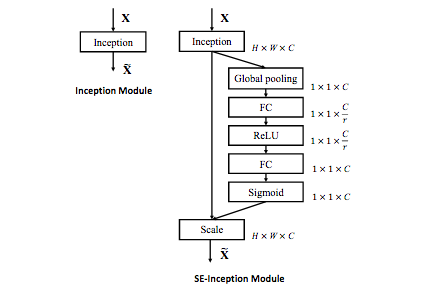
\includegraphics[width=4in]{csci-8110/hw-3/images/SENet_diagram.png}
    \caption{The schema of the original Inception module (left) and the SE-Inception module (right). From Hu, et al \cite{Hu2020Squeeze-and-ExcitationNetworks}.}
    \label{fig:diagram}
\end{figure}

\par Some research had to be done into how to get models to work properly in Keras. 
The format for this SENet block was informed primarily by the method used in the VGG16 source, which can be obtained by Ctrl + Clicking \lstinline{VGG16} in the Google Colab editor.
That format, generally, is as follows:

\begin{lstlisting}[language=Python]
# Block 1
x = layers.Conv2D(
  64, (3, 3), activation='relu', padding='same', name='block1_conv1')(
      img_input)
x = layers.Conv2D(
  64, (3, 3), activation='relu', padding='same', name='block1_conv2')(x)
x = layers.MaxPooling2D((2, 2), strides=(2, 2), name='block1_pool')(x)

# ... and so on
\end{lstlisting}

\par With this in mind, the SENet implementation as defined in Figure \ref{fig:diagram} was, relatively straightforwardly, implemented in code as follows:

\begin{lstlisting}[language=Python]
def SENet_impl(init, ratio=16):
  channel_axis = 1 if K.image_data_format() == "channels_first" else -1
  filters = init.shape[channel_axis]
  se_shape = (1, 1, filters)

  x = GlobalAveragePooling2D()(init)
  x = Reshape(se_shape)(x)
  x = Dense(filters // ratio, activation='relu', kernel_initializer='he_normal')(x)
  x = Dense(filters, activation='sigmoid', kernel_initializer='he_normal')(x)

  if K.image_data_format() == 'channels_first':
    x = Permute((3, 1, 2))(x)

  out = multiply([init, x])
  return out
\end{lstlisting}

\par A significantly more difficult task included getting the SENet implementation included in various locations of the VGG16 model, compiling the new model, training only the relevant layers,and finally getting predictions out of that model once it was compiled. These problems, and their resolutions, are discussed below.

\par Initially, to implement the SENet block into the model, the strategy was to use Keras' built-in \lstinline{Sequential} module, and then add layers from the original VGG16 model using the \lstinline{model.add()} function.
This created compatibility issues, since the \lstinline{SENet_impl()} function doesn't output a layer--it outputs the \textit{results} of several layer operations.
So, once again, inspiration was taken from VGG16, and a separate model was created altogether, again using the strategy of feeding one layer's output into the next layer:

\begin{lstlisting}[language=Python]
from tensorflow.keras import Model

# save original model for comparison later
model_copy = model

for il in range(len(model_copy.layers) - 1):
  if il == 0:
    xl = model_copy.layers[il].output
  else:
    xl = model_copy.layers[il](xl)
  # locations of pooling: 3,6,10,14,18
  # can change location accordingly
  if il == 3:
    xl = SENet_impl(xl)

# reduced softmax layer (to reduce number of considered categories to 10)
xl = Dense(10,activation='softmax')(xl)
\end{lstlisting}

\par Of note here: the assignment specifies that the SENet block should be placed after one of the Pooling layers at the end of each of VGG16's five blocks. 
To that end, the location of \lstinline{SENet_impl()} can be changed quickly using the \lstinline{if} statement on line 13. 
On a related note, the code on line 17 was added because predictions were consistently wrong after training--more on that below.

\par Training the model was difficult, because loading images into the model for training proved to be challenging.
Another classmate pointed out the built-in TensorFlow Datasets library, which was used to download the image set for imagenette and load it into the model as follows:

\begin{lstlisting}[language=Python]
# load imagenette images for processing
builder = tfds.builder('imagenette/160px')
builder.download_and_prepare()
datasets = builder.as_dataset(as_supervised=True)
train_data,test_data = datasets['train'],datasets['validation']

# define and prefetch training data
training_dataset = train_data.map(normalize_img, num_parallel_calls=tf.data.experimental.AUTOTUNE)
training_dataset = training_dataset.batch(128)
training_dataset = training_dataset.prefetch(tf.data.experimental.AUTOTUNE)

# define and prefetch training data
validation_dataset = test_data.map(normalize_img, num_parallel_calls=tf.data.experimental.AUTOTUNE)
validation_dataset = validation_dataset.batch(128)
validation_dataset = validation_dataset.prefetch(tf.data.experimental.AUTOTUNE)

# fit new data to train SENet and softmax layers
new_model.fit(training_dataset,
              validation_data=validation_dataset,
              batch_size=128,
              epochs=10)
\end{lstlisting}

\par Finally, the last difficulty encountered was in getting predictions out of the model.
This is the step mentioned above in the paragraph about constructing the updated model.
It was difficult to get proper predictions from the adjusted model because it was being run against all 1000 weighted classes of the imagenet dataset. 
Consistently incorrect predictions were produced from the model, as seen below:

\begin{figure}[H]
    \centering
    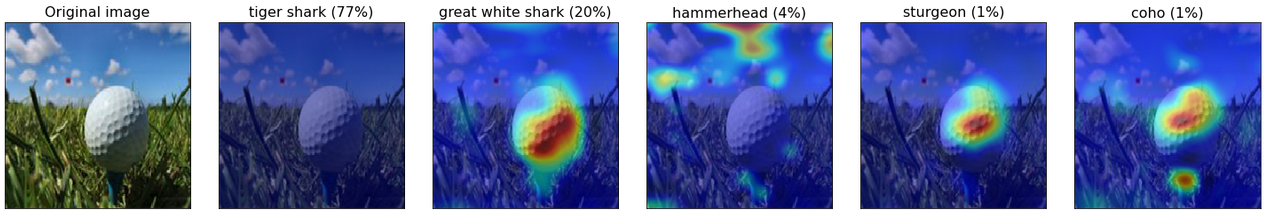
\includegraphics[width=6in]{csci-8110/hw-3/images/bad_predicts.png}
    \caption{A golf ball, or a tiger shark?}
    \label{fig:bad_predicts}
\end{figure}

\par Resolving this was difficult.
It was not immediately intuitive that the built-in Keras \lstinline{model.predict()} command wouldn't work.
Since the model was trained on ten categories of images, it turned out that too many categories were left to "predict" from.
Some code was developed to replace the built-in prediction function:

\begin{lstlisting}[language=Python]
input_title = 'golf'
img1 = load_img(f'/content/.../inputs/{input_title}.JPEG', target_size=(224, 224))
images = np.asarray([np.array(img1)])

counter = 0
preprocessed_images = preprocess_input(images)
image_titles = []
image_categories = []
for i in preprocessed_images:
  x = i.reshape((1, i.shape[0], i.shape[1], i.shape[2]))
  y = new_model.predict(x)
  y = y[0]
  max_y = np.max(y)
  # define location where prediction is (value of 1 in array, all other values 0)
  max_loc = np.where(y == max_y)
  # get appropriate prediction label
  # some very lazy fitting of these predictions to my grad-CAM params from HW 2
  predictions = imagenette_labels.get(max_loc[0][0])
  prediction_name = predictions
  image_titles.append(prediction_name)
  image_categories.append(find_cat_in_dict(prediction_name))
\end{lstlisting}

\par Compared against the smaller set of categories, outputs are more consistently correct. 
Note that grad-CAM visualizations never got to a working state in the new code but were useful--and entertaining--while investigating the problems with the initial predictions.

\par The final component of the assignment was feature mapping--this was actually fairly straightforward using some code adapted from an online blog post \cite{Brownlee2019HowNetworks}:

\begin{lstlisting}[language=Python]
# convert the image to an array
img = img_to_array(img1)
# expand dimensions so that it represents a single 'sample'
img = expand_dims(img, axis=0)
img = preprocess_input(img)

# get the last layer of SENet_impl (multiply)
layer_loc = 0
for layer in new_model.layers:
    if "multiply" in layer.name:
      print(i, layer.name)
      break
    layer_loc = layer_loc + 1

# get outputs from AFTER the SENet block
featmap_model = Model(inputs=new_model.inputs, outputs=new_model.layers[layer_loc].output)
feature_maps = featmap_model.predict(img)

pyplot.figure(figsize=(16,16))
square = 8
ix = 1
for _ in range(square):
	for _ in range(square):
		# specify subplot and turn of axis
		ax = pyplot.subplot(square, square, ix)
		ax.set_xticks([])
		ax.set_yticks([])
		# plot filter channel in grayscale
		pyplot.imshow(feature_maps[0, :, :, ix-1], cmap='gray')
		ix += 1
plt.savefig()

\end{lstlisting}

\par This code is run twice--once for the layer preceding the SENet block, and once for the last layer of the SENet block. Outputs are discussed in \nameref{model_obvs}.

\subsection{Model Observations} \label{model_obvs}
\par The layer observations were a useful tool in determining how the SENet implementation works when applied in the context of a model like VGG16.
Using the code described in the \nameref{impl} section, it is possible to obtain a pair of image collections representing the filters at the layer in question. Take, for example, given the image of a golf ball below:

\begin{figure}[H]
    \centering
    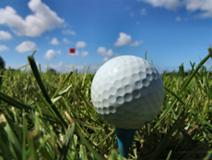
\includegraphics[width=2in]{csci-8110/hw-3/images/golf.JPEG}
    \caption{Golf ball input}
    \label{fig:gas_input}
\end{figure}

\par When the SENet block is inserted after the pooling layer in block 1, the results can be seen in the image collections below:

\begin{figure}[H]
    \centering
    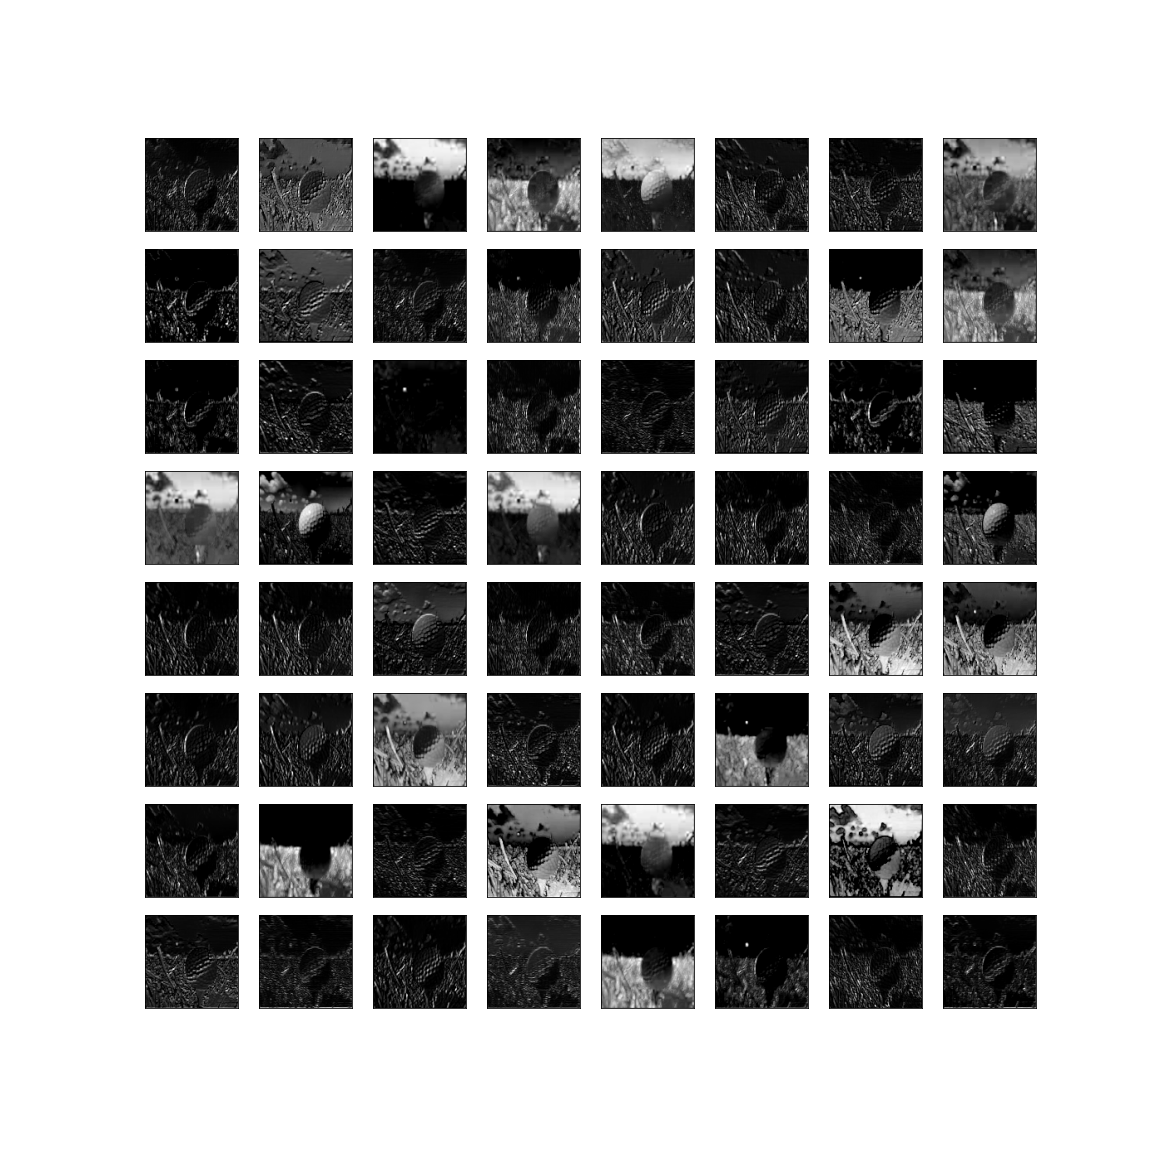
\includegraphics[width=6in]{csci-8110/hw-3/images/golf-pre-SENet-block1_pool-2020-11-06 02_39_48.350774_output.png}
    \caption{Golf ball feature map after \lstinline{block1_pool}, before SENet}
    \label{fig:golf_1_pre}
\end{figure}

\begin{figure}[H]
    \centering
    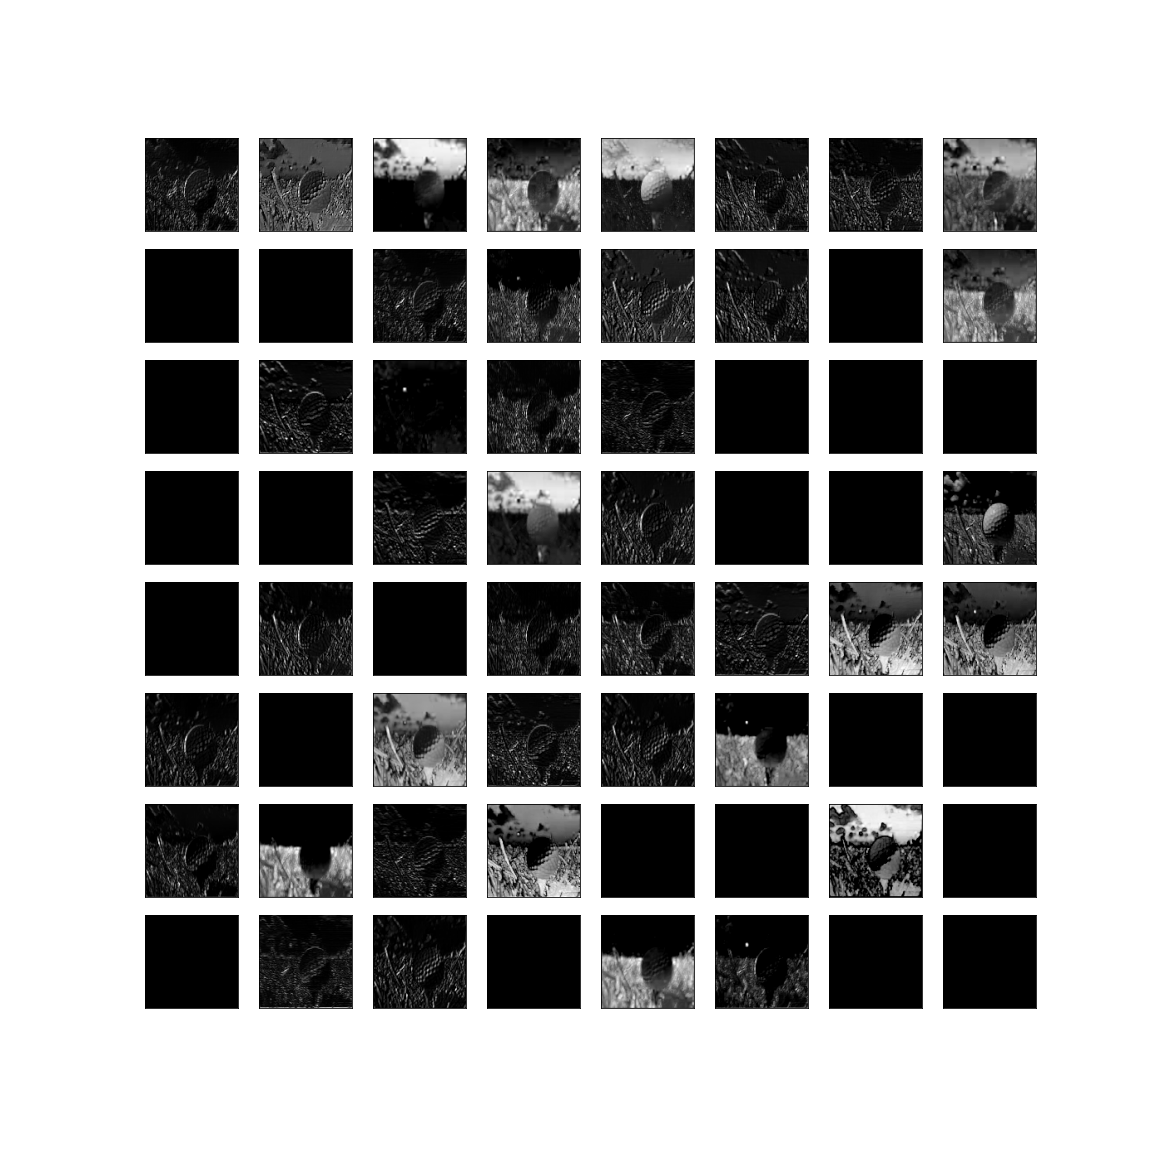
\includegraphics[width=6in]{csci-8110/hw-3/images/golf-post-SENet-block1_pool-2020-11-06 02_39_51.127362_output.png}
    \caption{Golf ball feature map before \lstinline{block2_conv1}, after SENet}
    \label{fig:golf_1_post}
\end{figure}

\par For brevity, more model results can be found in \nameref{modelouts}.
\par Some observations can be derived from feature mapping, in general. 
The impact of the SENet block appears to be visible in these images--the block appears to direct attention more toward relevant parts of the image.
This is observable in figures \ref{fig:golf_1_pre} and \ref{fig:golf_1_post}, above, where more details are visible in the pre-SENet feature maps than the post-SENet feature maps.
It follows, then, that the SENet block does indeed direct attention toward the more relevant parts of the image, aiding the model generally.

\par Also of note in the feature maps is that the SENet block appears to be more consequential placed in the middle of the VGG16 model, rather than earlier or later.
This can be seen in the images listed in \nameref{modelouts}--there are more differences in the comparisons when SENet is placed after block 3 than in the comparisons when SENet is placed after block 1 or 5.

\section{Conclusions}
\par This was a difficult--but rewarding--assignment. Going in, it wasn't expected that so much of this assignment would hinge upon properly understanding and implementing model predictions.
Given prior assignments, this probably shouldn't have been a surprise--copying layer details from a paper is relatively easy.
Implementing them in the context of a model, or using different data, is much harder.

\par All said, despite issues training and obtaining classifications from the updated models, this was a useful exercise toward developing the continued understanding of attention and image classification using convolutional neural networks.
The concepts of training models for data is still much hazier than the process of identifying features in examples--hopefully more time can be devoted to understanding the mechanics of training models more effectively.

\bibliographystyle{unsrt}
\bibliography{references}

\begin{appendices}
\newpage
\section{Complete Code Listing} \label{codelist}
\lstinputlisting[language=Python]{8110_hw3.py}


\newpage
\section{Model Output Listing} \label{modelouts}
\begin{figure}[H]
    \centering
    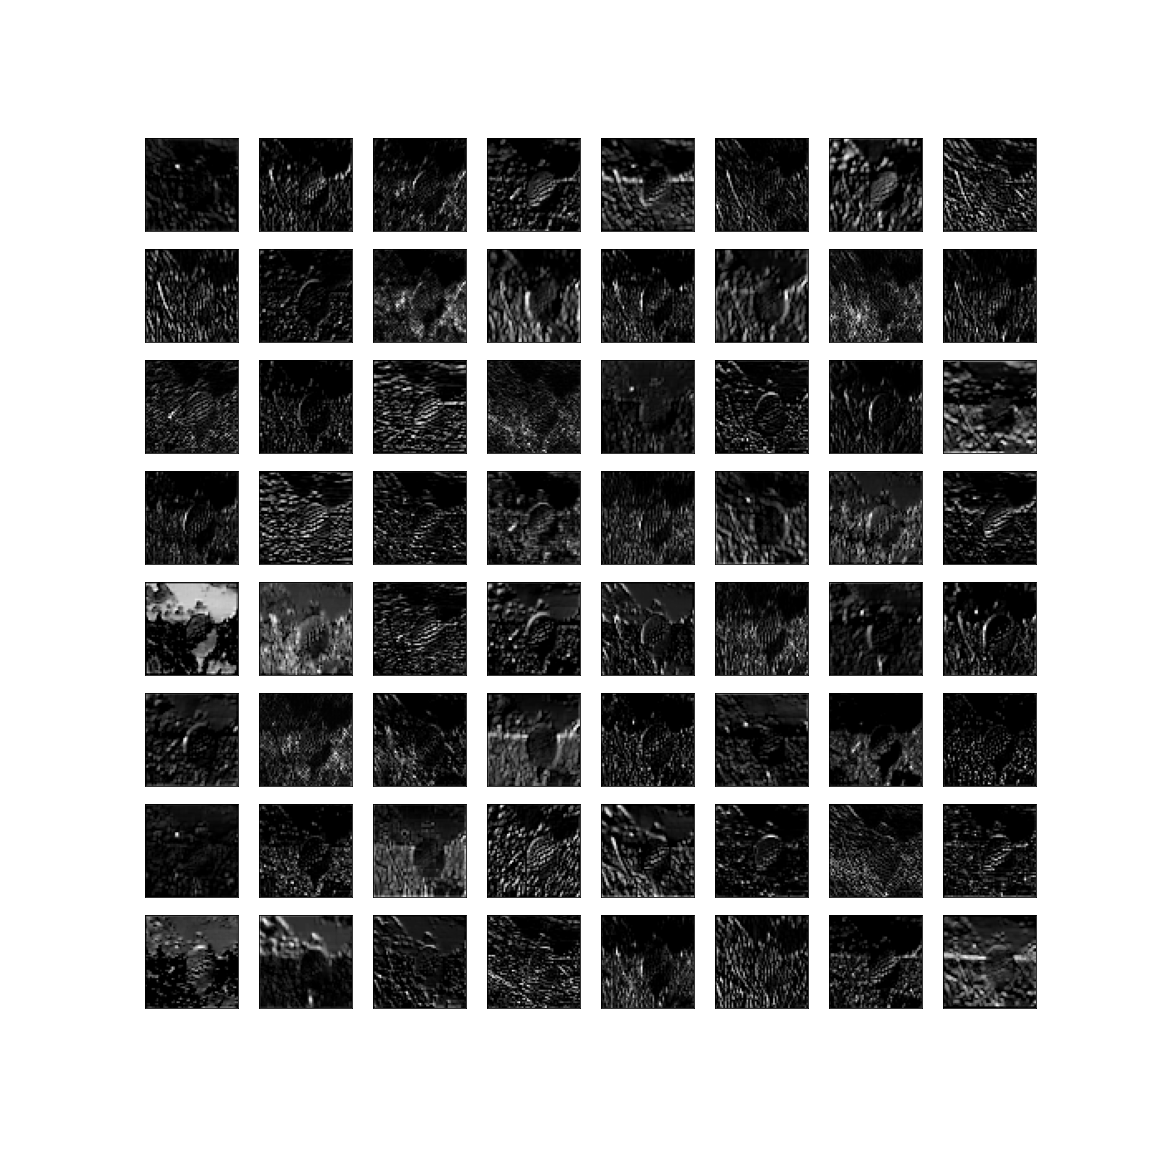
\includegraphics[width=3in]{csci-8110/hw-3/images/golf-pre-SENet-block2_pool-2020-11-05 18_25_06.663590_output.png}
    \caption{Golf ball feature map after \lstinline{block2_pool}, before SENet}
    \label{fig:golf_2_pre}
\end{figure}

\begin{figure}[H]
    \centering
    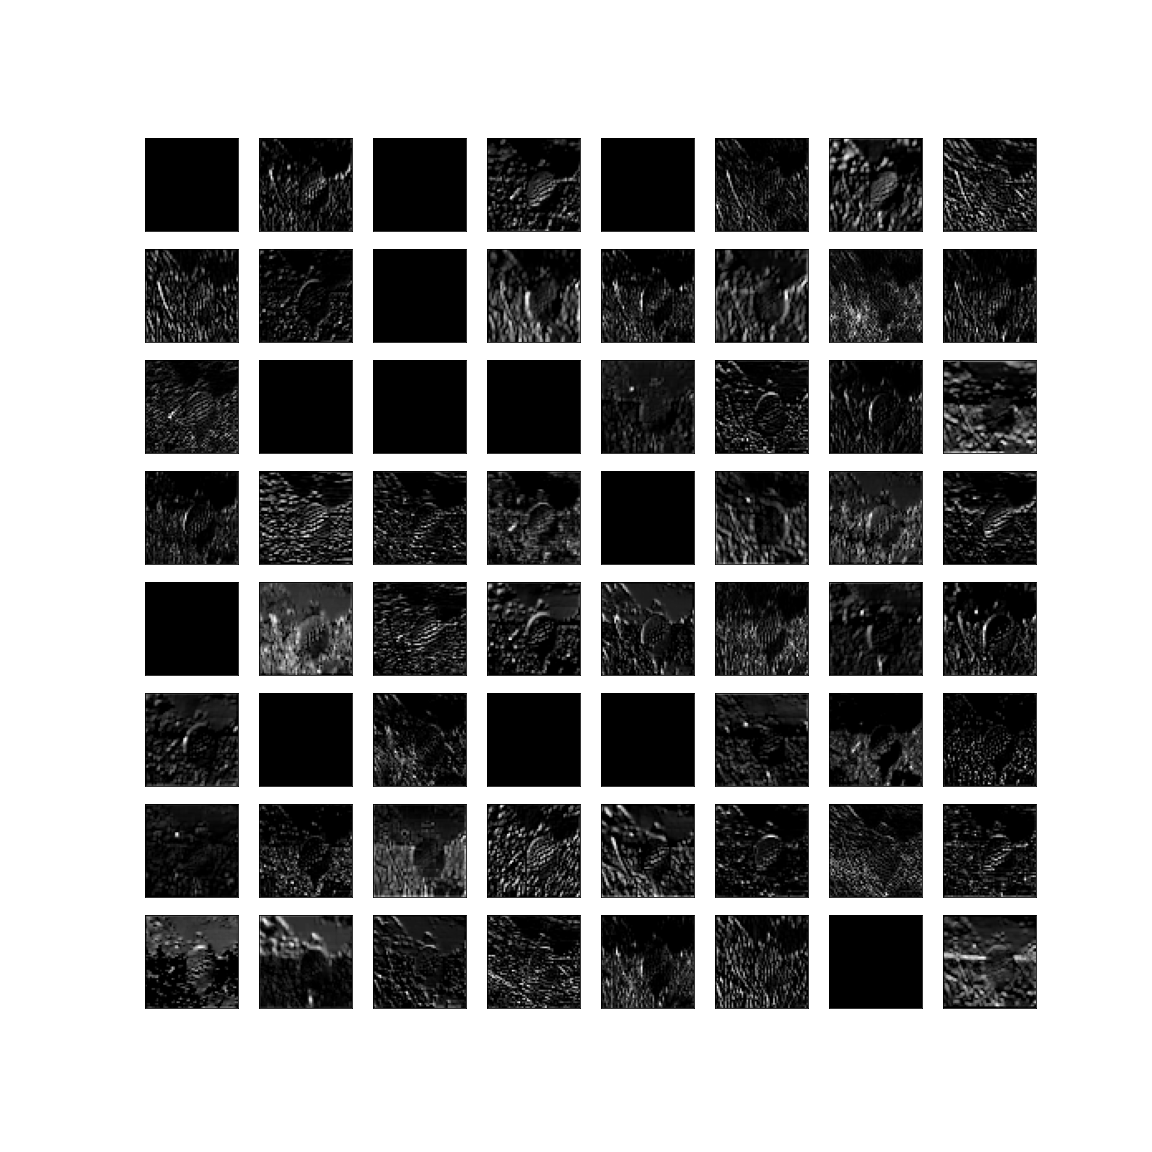
\includegraphics[width=3in]{csci-8110/hw-3/images/golf-post-SENet-block2_pool-2020-11-05 18_25_10.151699_output.png}
    \caption{Golf ball feature map before \lstinline{block3_conv1}, after SENet}
    \label{fig:golf_2_post}
\end{figure}
\begin{figure}[H]
    \centering
    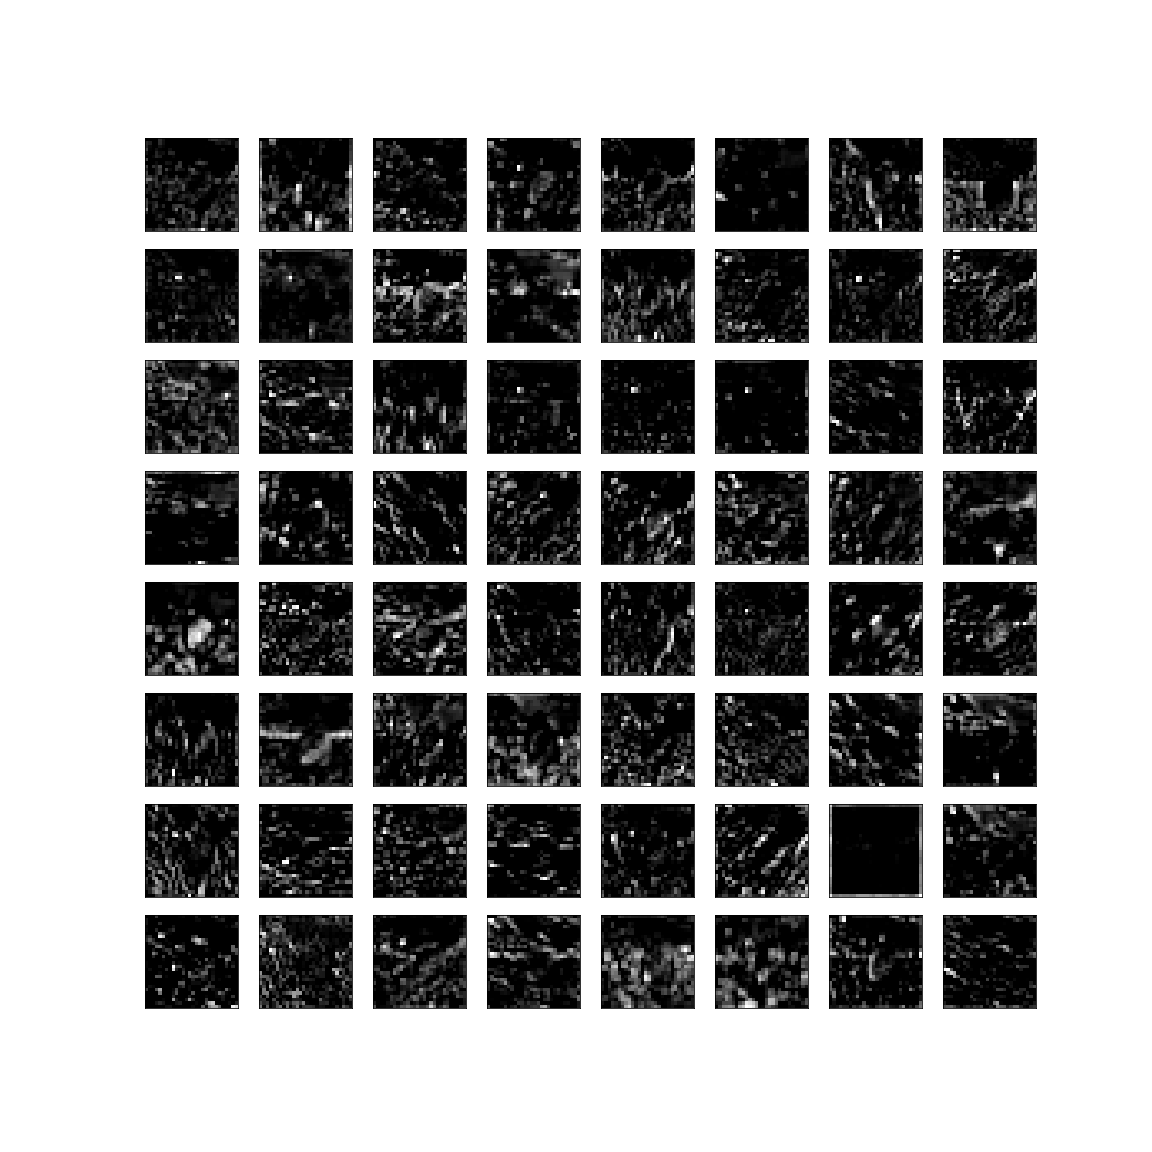
\includegraphics[width=3in]{csci-8110/hw-3/images/golf-pre-SENet-block3_pool-2020-11-05 18_29_43.542902_output.png}
    \caption{Golf ball feature map after \lstinline{block3_pool}, before SENet}
    \label{fig:golf_3_pre}
\end{figure}

\begin{figure}[H]
    \centering
    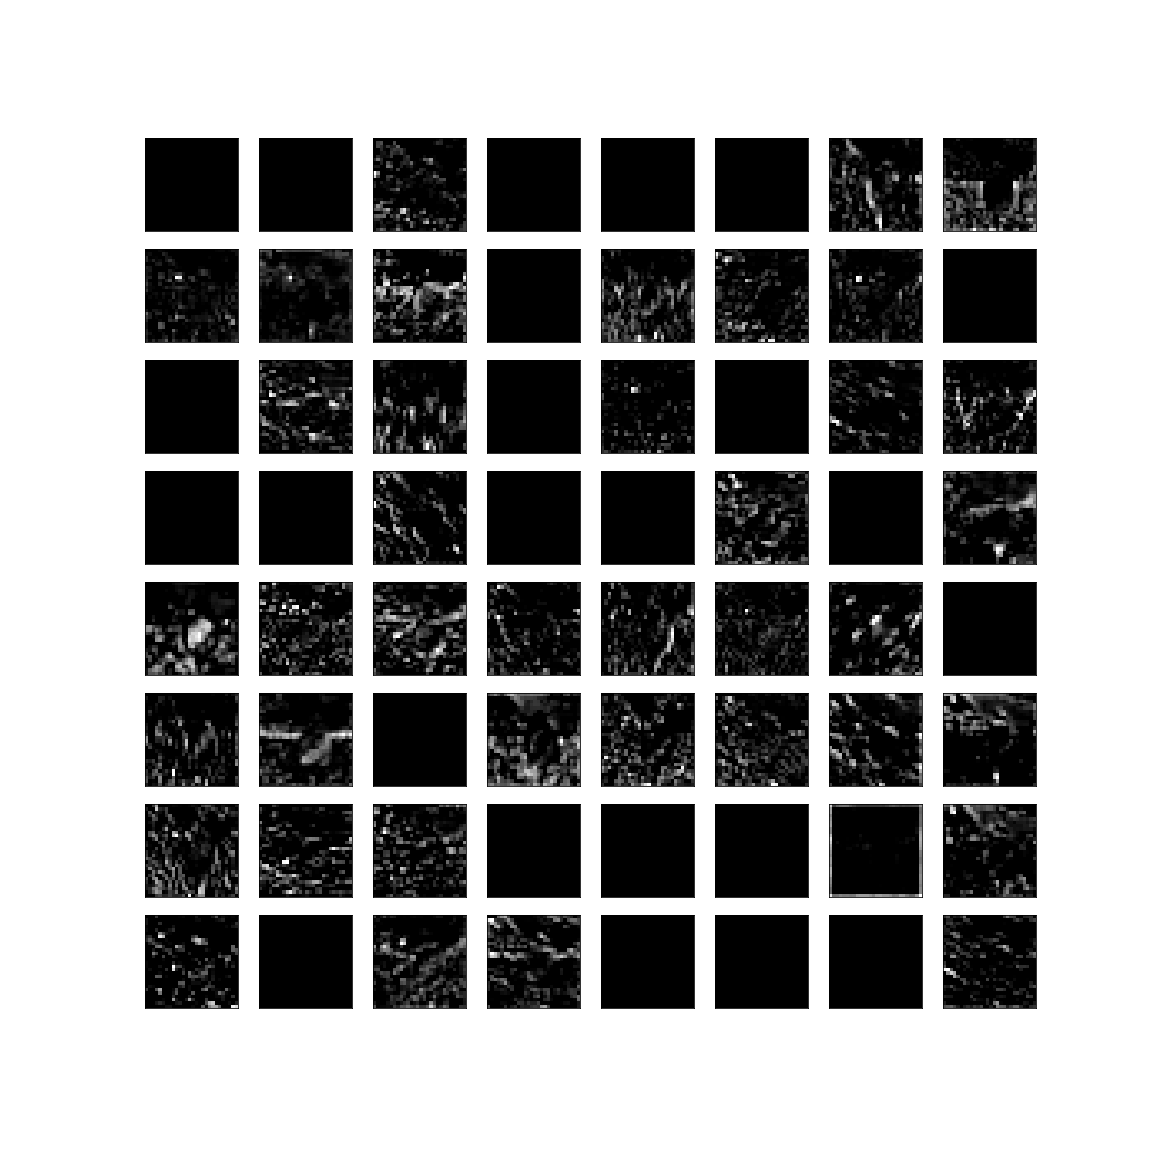
\includegraphics[width=3in]{csci-8110/hw-3/images/golf-post-SENet-block3_pool-2020-11-05 18_29_46.031795_output.png}
    \caption{Golf ball feature map before \lstinline{block4_conv1}, after SENet}
    \label{fig:golf_3_post}
\end{figure}
\begin{figure}[H]
    \centering
    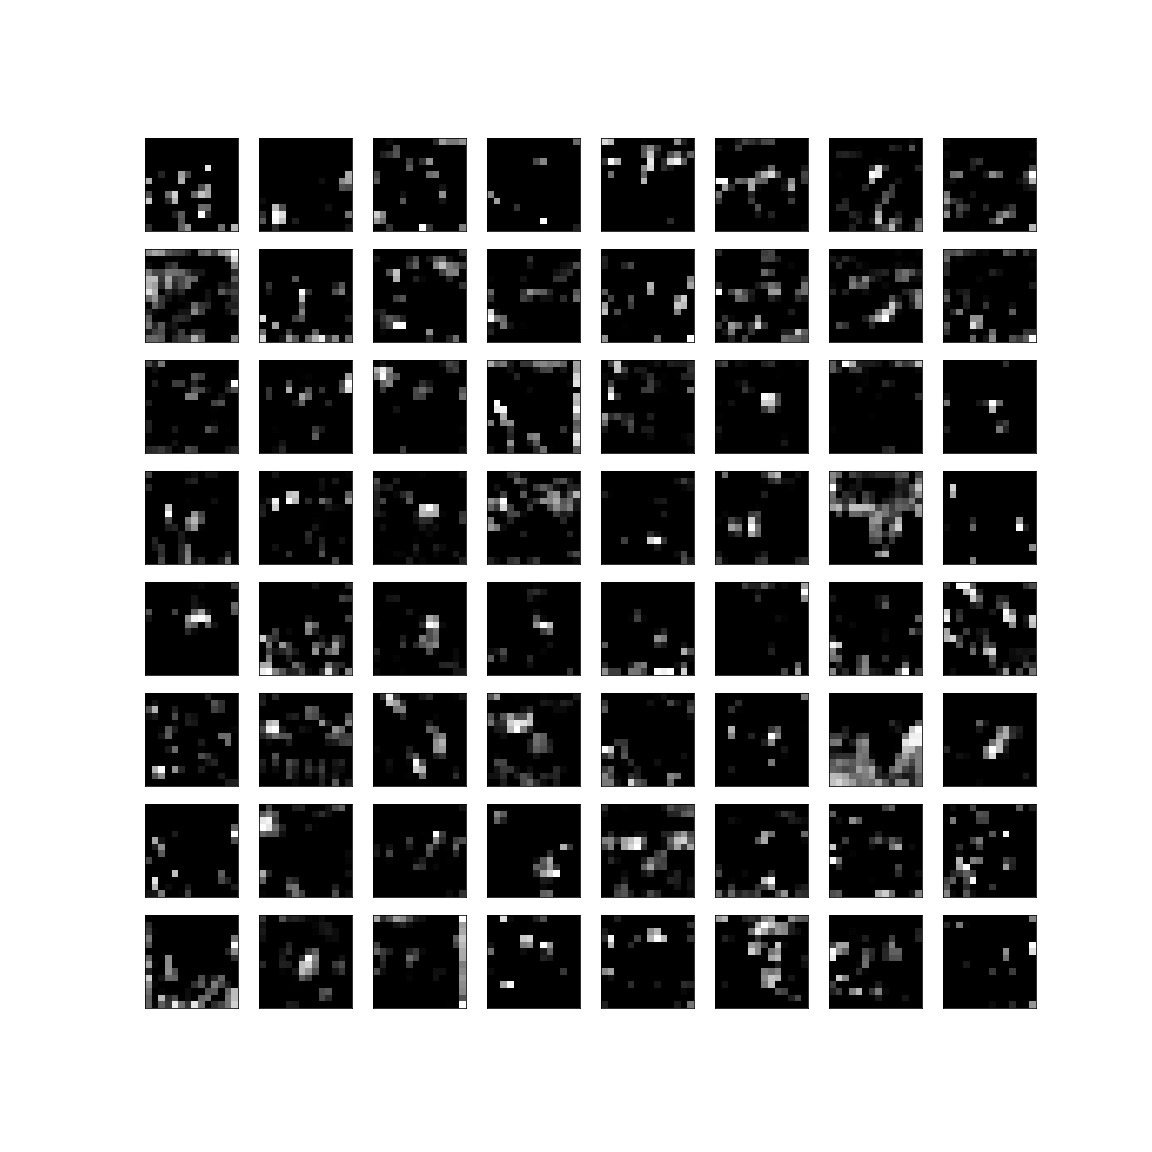
\includegraphics[width=3in]{csci-8110/hw-3/images/golf-pre-SENet-block4_pool-2020-11-05 18_35_31.491006_output.png}
    \caption{Golf ball feature map after \lstinline{block4_pool}, before SENet}
    \label{fig:golf_4_pre}
\end{figure}

\begin{figure}[H]
    \centering
    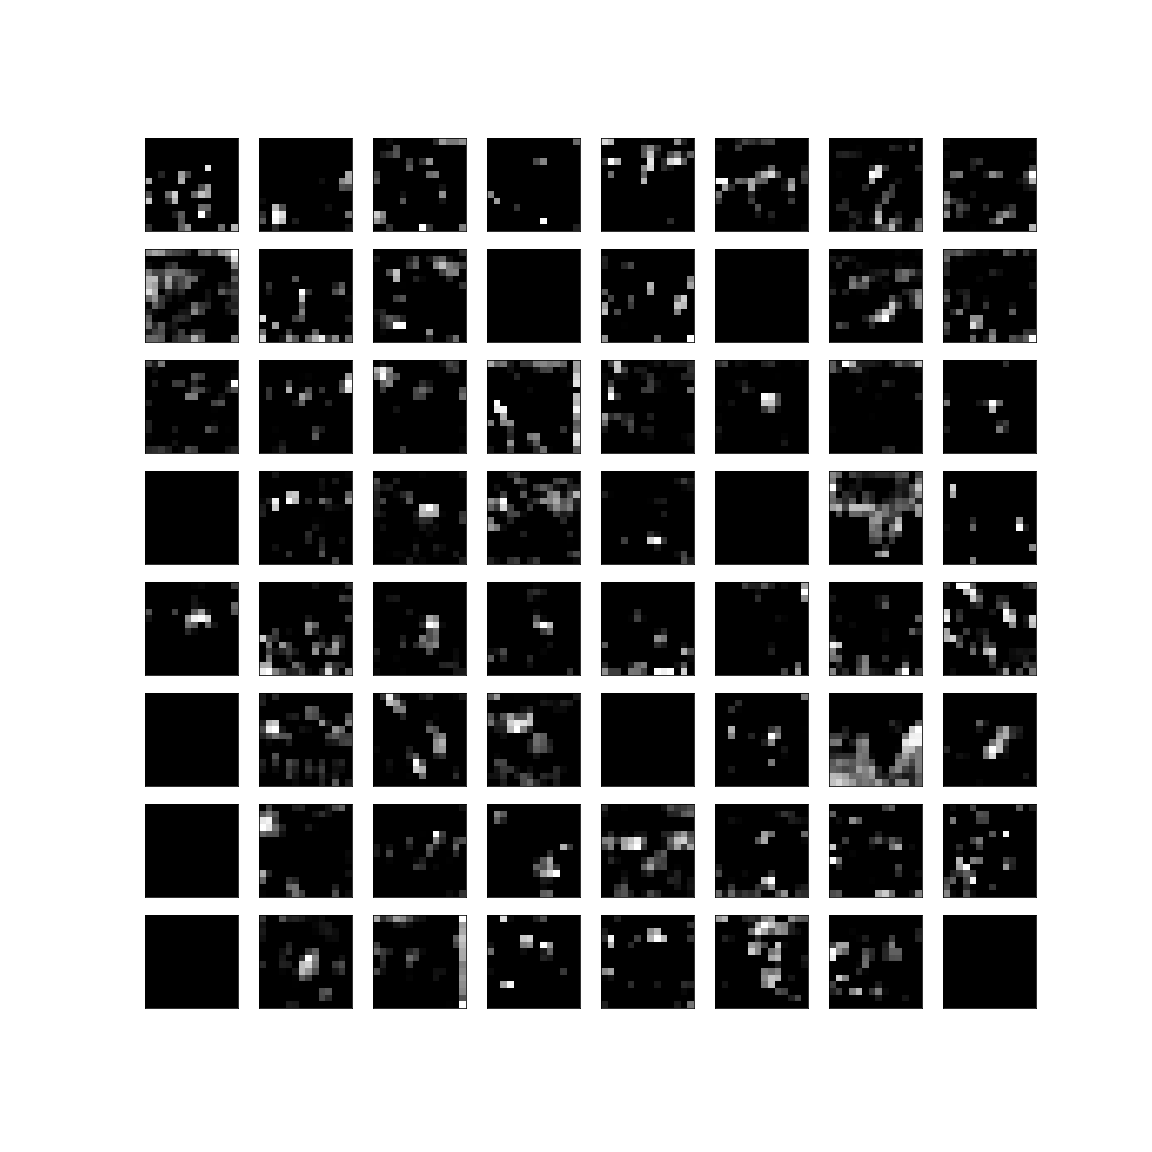
\includegraphics[width=3in]{csci-8110/hw-3/images/golf-post-SENet-block4_pool-2020-11-05 18_35_33.867099_output.png}
    \caption{Golf ball feature map before \lstinline{block5_conv1}, after SENet}
    \label{fig:golf_4_post}
\end{figure}
\begin{figure}[H]
    \centering
    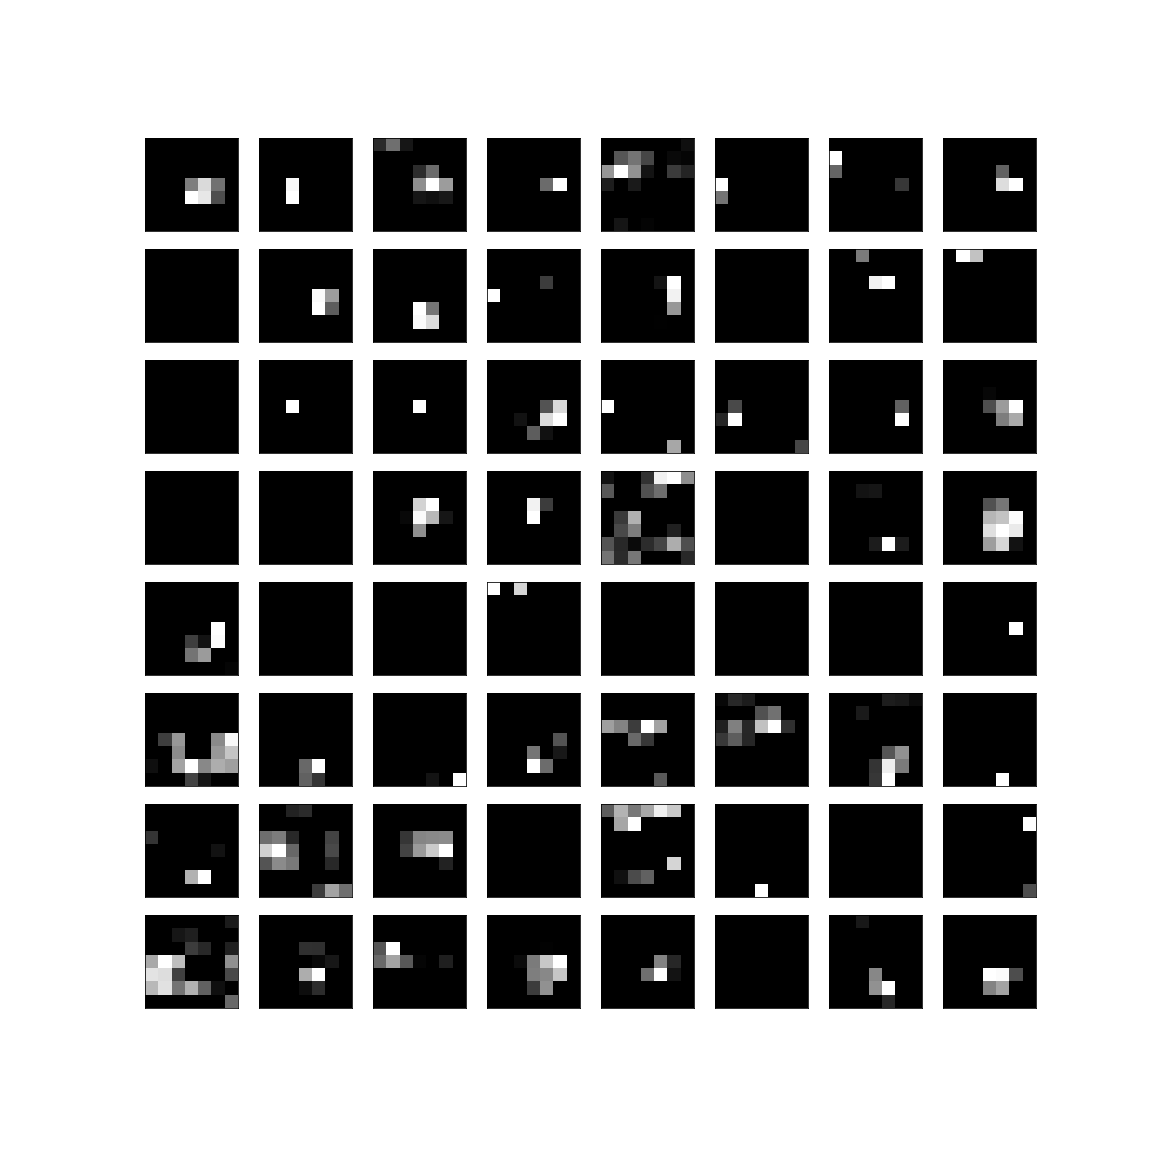
\includegraphics[width=3in]{csci-8110/hw-3/images/golf-pre-SENet-block5_pool-2020-11-05 18_44_09.014537_output.png}
    \caption{Golf ball feature map after \lstinline{block5_pool}, before SENet}
    \label{fig:golf_5_pre}
\end{figure}

\begin{figure}[H]
    \centering
    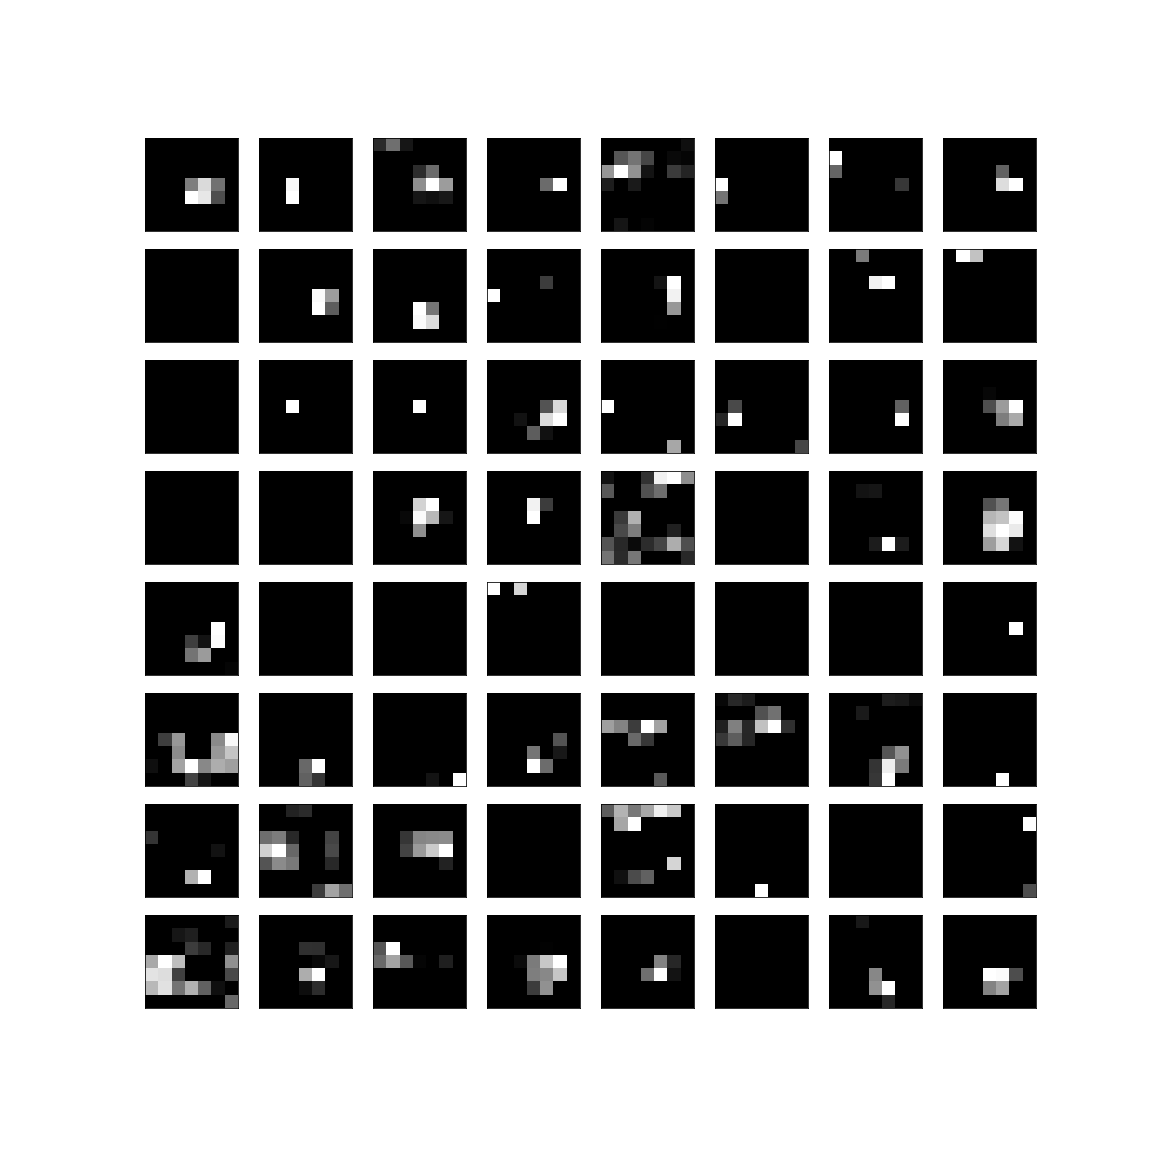
\includegraphics[width=3in]{csci-8110/hw-3/images/golf-post-SENet-block5_pool-2020-11-05 18_44_11.709641_output.png}
    \caption{Golf ball feature map before \lstinline{flatten}, after SENet}
    \label{fig:golf_5_post}
\end{figure}

\par NOTE: to keep this report from being 50 pages long, a complete set of images can be found on the UNO Google Drive by \href{https://drive.google.com/drive/folders/1thcSPIT0QEPa8tnmXHmzTmB66VScgZe-?usp=sharing}{clicking here}. They should be appropriately timestamped.

\end{appendices}

\end{document}